\documentclass[a4paper,12pt]{article}
\usepackage[verbose,a4paper,tmargin=3cm,bmargin=3cm,lmargin=2.5cm,rmargin=2.5cm]{geometry}
\usepackage[utf8]{inputenc}
% \usepackage{polski}
\usepackage{amsmath}
\usepackage{graphicx}
\usepackage{siunitx}
\usepackage{float}
\usepackage{lastpage}
\usepackage{mathtools}
\usepackage{caption}
\usepackage{subcaption}
\usepackage{multirow}
\usepackage{wrapfig}
\usepackage{url}
\usepackage[table,xcdraw]{xcolor}
\usepackage{booktabs}
\usepackage{adjustbox}
\usepackage{pdflscape}

%foot
\usepackage{fancyhdr}
\pagestyle{fancyplain}
\fancyhf{}
\renewcommand{\headrulewidth}{0pt}
\renewcommand{\footrulewidth}{0.4pt}
\fancyfoot[L]{Patryk Lisik, Mateusz Borowiec, Assignment \# 1}
\fancyfoot[R]{\thepage\ / \pageref{LastPage}}

\begin{document}
\begin{titlepage}
\vspace{3cm}

\begin{minipage}{0.33 \textwidth}
\begin{flushleft}
\large
% Imię i nazwisko:\\
\textsc{Patryk Lisik}
\end{flushleft}
\end{minipage}
\hspace{0.2\textwidth}
\begin{minipage}{0.33 \textwidth}
\begin{flushleft}
\large
% Imię i nazwisko:\\
\textsc{Mateusz Borowiec}
\end{flushleft}
\end{minipage}

\vspace{2cm}

{\center\huge\bfseries Agile Methods \par}

\vspace{1.5cm}
{\center\huge\bfseries Assignment \#1\par}

\end{titlepage}
\section{Introduction}

Ability to process large quantity of data has always been one of the main forces that shapes the world.
With growth of human organization, grows demand for computation.
% some hsitory of computation ??
Before computing machines, humans had to perform all calculations by themselves, sometimes with small support of tools like an abacus or a slide rule. 
Modern English word "Computer" still refers to a person who performs calculations and computations \cite{DictioanryComputer}.
For this very reason invention of a transistor and  processor, that outperformed room of people computing by orders of magnitude, revolutionized the world.
\begin{wrapfigure}{l}{0.35\textwidth}
    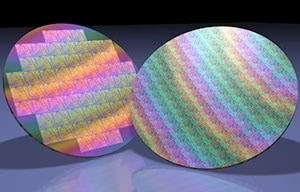
\includegraphics[width=0.9\linewidth]{silicon_waffers.png}
    \caption{Printed silicon wafers. Source: \cite{hitachiHightechManufactering}}
    \label{img:silicon-waffers}
\end{wrapfigure}
Invention of transistor spawned whole new industry -- the semiconductor industry. 
Every semiconductor starts as large bar of almost pure silicon shown on figure \ref{img:monocrystal-silicon}, that is sliced in circular wafers \cite{ASMLSemiconductorProduction}.
Such wafers are shown on figure \ref{img:silicon-waffers}.
In the step circuit is printed on to the wafer in process, called lithography.
Lithography process itself is so complex and expensive, that  even mega companies like Samsung or Intel do not make lithography machines themselves.
They cooperate with ASML, who provides such equipment  \cite{ASMLAnnualReport}.
and even need to cooperate with ASML to stay competitive.
Closer look on picture \ref{img:silicon-waffers} shows that wafer has some free space around the edges, as it is impossible to cover the whole circle with squares entirely.  
Not all semiconductors are made equal. 
Key characteristics of chip come from two sources -- circuit design and transistor technology. 
Circuit design or architecture describes how electronic signals are processed after chip is made. 
Transistor technology or node usually refers to the size of single transitory. 
Smaller transistors can be packed up denser in the chip of same size, with better thermal characteristic.  
There is no standardized method to refer to transistor size hence differences between companies.
In Intel's 14 nm node, 14 nm does not refer to any physical part of transistor or integrated circuit, can not be compared to Samsung or TSMC process technology.

\begin{wrapfigure}{l}{0.35\textwidth}
    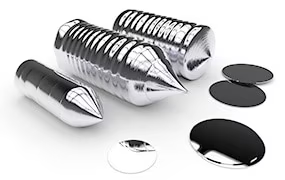
\includegraphics[width=0.9\linewidth]{monocrystal_silicon.png}
    \caption{Mono-crystal of silicon that id used in semiconductor manufacturing. Source: \cite{hitachiHightechManufactering}}
    \label{img:monocrystal-silicon}
\end{wrapfigure}


This work describes business model of TSMC (Taiwan Semiconductor Manufacturing Company Limited).
Before mentioned company entered the market in 1987 as one of the very first company that manufactures semiconductors but does not design them \cite{TSMCwebCompanyProfile}.
TSMC does not compete in  semiconductor products markets like IoT, smartphone, HPC (high performance computing) etc.
This ensures that it is in TSMC and its customers best interest for a product to succeed.
This is very different from Apple and Samsung cooperation.
Samsung competes in semiconductor products market and used to manufacture its main competitor(Apple) phone chip, which may have resulted in potential frictions, as Samsung would have benefited from worsening Apples chip.
Not competing in market enables TSMC to entirely focus on advancing production process, developing best designing tools and ensuring availability of factories. 

\tableofcontents




\section{CANVAS Business Model}
Table \ref{tab:tsmc-canvas} show CANVAS analysis of TSMC while the following sections dives into deeper details about particular segments of analysis.  
\begin{table}[h]
\begin{adjustbox}{max width=\textwidth}
\begin{tabular}{lllll}
\rowcolor[HTML]{FFCCC9} 
\cellcolor[HTML]{FFCCC9}Key Partners & Key Activities & \cellcolor[HTML]{FFCCC9}Value Propositions & Customer Relationships & Customer Segments \\
ASML &
  Printing wafers &
  Semiconductors design tools &
  Business to business &
  Automotive \\
FST &
  Storing raw materials &
  Bleeding edge production node &
   &
  Digital Consumer Electronics \\
GlobalWafers &
  Storing products &
  Reliability &
   &
  High-Performance Computing \\
SEH &
  R\&D &
   &
   &
  Internet of Things \\
Siltronic &
  \cellcolor[HTML]{FFCCC9}Key Resources &
   &
   &
  Smartphones \\
SK siltron &
  Raw silicon wafers &
   &
  \cellcolor[HTML]{FFCCC9}Channels &
   \\
SUMCO &
  Chemicals &
   &
  Corporate offices &
   \\
Air Liquide &
  Photoresist &
    &
   Website &
   \\
BASF &
  Water &
     &
   Email &
   \\
DuPont &
  Gases &
    &
   Press center &
   \\
Entegris &
  Slurry &
    &
   Business contacts &
   \\
Fujifilm Electronic Materials &
  Pad &
   &
   Plants and production sites &
   \\
Kanto PPC &
  Disk &
   &
   &
   \\
Kuang Ming &
  Lithography machines &
   &
   &
   \\
Merck &
  Human resources &
   &
   &
   \\
RASA &
   &
   &
   &
   \\
Shiny &
   &
   &
   &
   \\
Tokuyama &
   &
   &
   &
   \\
Wah Lee &
   &
   &
   &
   \\
3M &
   &
   &
   &
   \\
Fujifilm Electronic Materials &
   &
   &
   &
   \\
JSR &
   &
   &
   &
   \\
Nissan &
   &
   &
   &
   \\
Shin-Etsu Chemical &
   &
   &
   &
   \\
Sumitomo Chemical &
   &
   &
   &
   \\
T.O.K. &
   &
   &
   &
   \\
Air Liquide &
   &
   &
   &
   \\
Air Products &
   &
   &
   &
   \\
Central Glass &
   &
   &
   &
   \\
Entegris &
   &
   &
   &
   \\
Linde LienHwa &
   &
   &
   &
   \\
Praxair &
   &
   &
   &
   \\
SK Materials &
   &
   &
   &
   \\
Taiwan Material Technology &
   &
   &
   &
   \\
Taiyo Nippon Sanso &
   &
   &
   &
   \\
3M &
   &
   &
   &
   \\
AGC &
   &
   &
   &
   \\
Cabot Microelectronics &
   &
   &
   &
   \\
DuPont &
   &
   &
   &
   \\
Fujibo &
   &
   &
   &
   \\
Fujifilm Electronic Materials &
   &
   &
   &
   \\
Fujimi &
   &
   &
   & \multicolumn{1}{l}{\cellcolor[HTML]{FFCCC9}Revenue streams}
   \\ 
\multicolumn{1}{l}{\cellcolor[HTML]{FFCCC9}Cost structure} &
   & 
   &
   &  Wafer sales 
   \\  beyond scope of this work
 &
   & 
   &
   & 
  
\end{tabular}
\end{adjustbox}
\caption{CANVAS analysis of TSMC based on their annual report \cite{TSMCAnnualReport}}
\label{tab:tsmc-canvas}
\end{table}

\subsection{Customer Segments}
Design and production of semiconductors is an expensive and labor-heavy endeavour, therefore TSMC provides services exclusively to other large business customers. 
In 2021 TSMC manufactured  products for 535 different customers \cite{TSMCAnnualReport}, meaning that they cannot be boxes into typical groups like mass or niche market. 
In figure \ref{img:net-revenue-by-client}, top TSMC client can be seen. 
Top 12 clients constitutes about 49\%  revenue, showing steep Pareto like distribution.
This work takes more individualized approach, splitting top clients into groups. 

Apple is TSMC's strategic customer generating one fourth of TSMC revenue and its client segment on its-own.
In 2017 chief operating officer Jeff Williams thanked TSMC for investing 9 billion USD and 6000 people working around a clock for 11 month in Tainan fab \cite{AppleOnTSMCInvestment}.
Not many companies can afford financial commitment like that, even less would bet 9 billion USD on other company.
In those 11 month TSMC supplied Apple with more then 500 million chips. 
Since then TSMC is Apple's only silicon manufacturer.
TSMC has accommodated its node improvement releases with roll out of new Apple devices every year.
Before cooperation with Apple new node was deployed when it was ready.
Apple needed improved SoC (system on chip) every year and that forced more gradual approach to new production process improvement. 
At its prime Intel\footnote{14 nm node took 4 years to improve upon and it is thought to be the end of tick-tock} was shrinking node in about every two years it was known as tick-tock strategy \footnote{Not to be confused with mobile app with short videos}.
Apple is always an early adopter of new risk-node and first customer been able to allocate high volume production of latest process \cite{AppleBookAll5nm}. 


\begin{wrapfigure}{}{0.65\textwidth}
    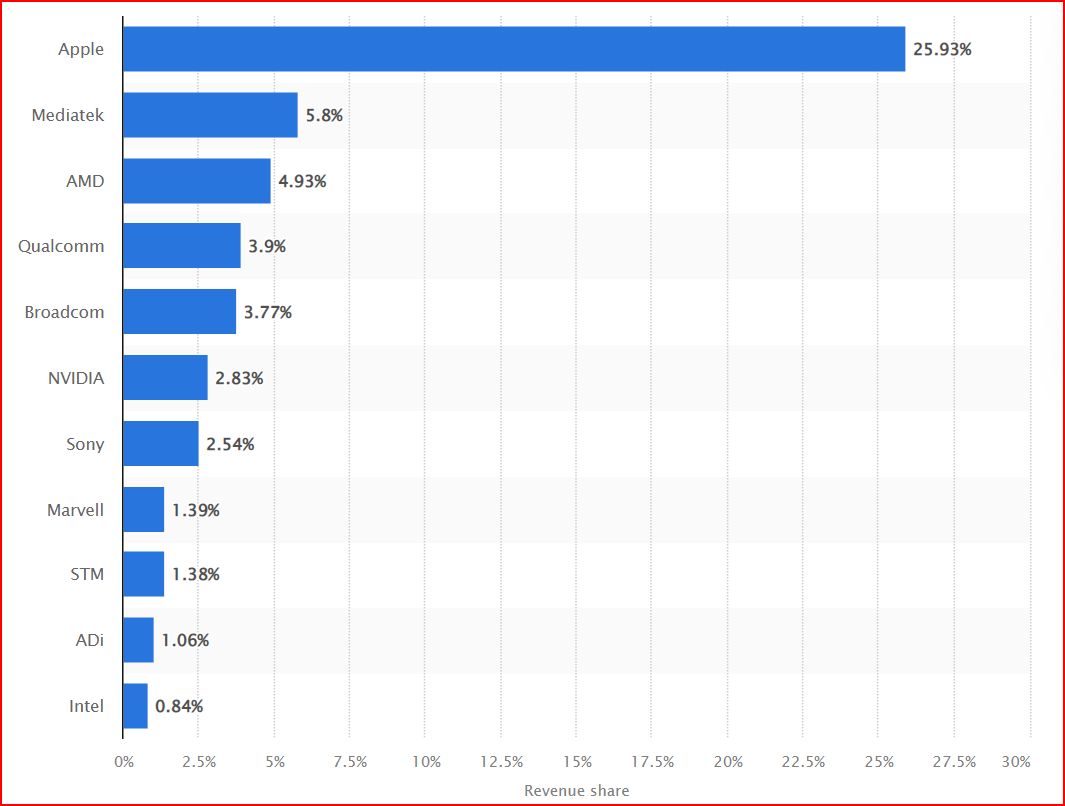
\includegraphics[width=0.9\linewidth]{TSMC_revenue_share.png}
    \caption{TSMC's clients by revenue. Data source: \cite{TSCMClientsByRevenue}}
    \label{img:net-revenue-by-client}
\end{wrapfigure}

Just behind Apple are high performance computing clients like AMD, NVIDIA, Sony.
Those companies are producing personal devices like processors, graphic cards, game consoles or other server and data center related products. 
Those product are competing in market by increasing performance, reducing power draw or increasing life-span.

Third segment contains companies producing chips that are integrated in other devices or solutions but not sold directly to customers. Those are arm processor companies like Qualcomm and Mediatek, data-center and cloud infrastructure providers like Marvell or Broadcom, integrated circuits makers ADi.


\subsection{Value Propositions}
This section describes what TSMC company offers to customers that sets them apart from what their competitors offer. These are the benefits that the customer will receive.
% First will be being "the most advanced and largest technology and foundry services provider to fabless companies".
% It means that TSMC aims to be the best in its activity, which is performing outsourcing for various companies.
% Next, "To serve and support our customer's manufacturing needs" is self-explanatory. It means that TSMC handles whole semiconductor manufacturing process for fabless companies.

Opposite to other top foundry players, like Intel and Samsung, TSMC does not compete in semiconductor device market. 
That ensures that company outsourcing chip making does not have to reveal its potential product to its competitor.
Product success is in TSMC and its customer best interest as it will drive further orders. 

Key part of TSMC business model is its ability to provide high volume production on cutting edge node. 
Using top production technology gives companies' product competitive advantage in computing speed or power and thermal efficiency.
Better production technology give more then chip architecture improvement in graphic card or smartphone market. 

\subsection{Channels}
Channels represent ways to get new customers for TSMC. For example, it can be business contacts and company website, which are probably the most effective way for enterprise existing in such niche. Other, like e-mail or press are less effective.

\subsection{Customer Relationships}
For its size TSMC does not have large customer base, enabling them to cooperate closer with every one of its customers.
TSMC has established a dedicated service team that strives to provide world-class services to support customers in product design, mask making, wafer manufacturing, and backend services, hence TSMC can increase customer satisfaction and win customer trust in order to maintain sales and profitability of the company.
Clients can request engineering collaboration including engineering lots, wafer yields and wafer acceptance test analysis, as well as quality and reliability data.
Logistics collaboration includes 24/7 information on wafer fabrication, backend processes and order shipments. 
TSMC complies with applicable regulations and international standards in terms of customer information protection and has
received ISO 27001 international information security certification.

\subsection{Revenue Streams}


TSMC-made semiconductors serve a global customer base that includes a wide
range of applications. 
Figure \ref{img:net-revenue-by-platform} shows TSMC's most profitable markets are smartphones and high performance computing (HPC).
Figure \ref{img:net-revenue-by-technology} shows that most advanced nodes (5 nm and 7 nm) make up to 49\% of income.  
As mentioned before Apple is TSMC's biggest customer, paying top dollar for leading-edge silicon products. 
One the biggest ARM and therefore basically smartphone chips suppliers Qualcomm and Mediatek are producing their products with TSMC.
It should be no surprise that smartphone market accounts for 44\% of TSCM income.


\begin{wrapfigure}{r}{0.7\textwidth}
    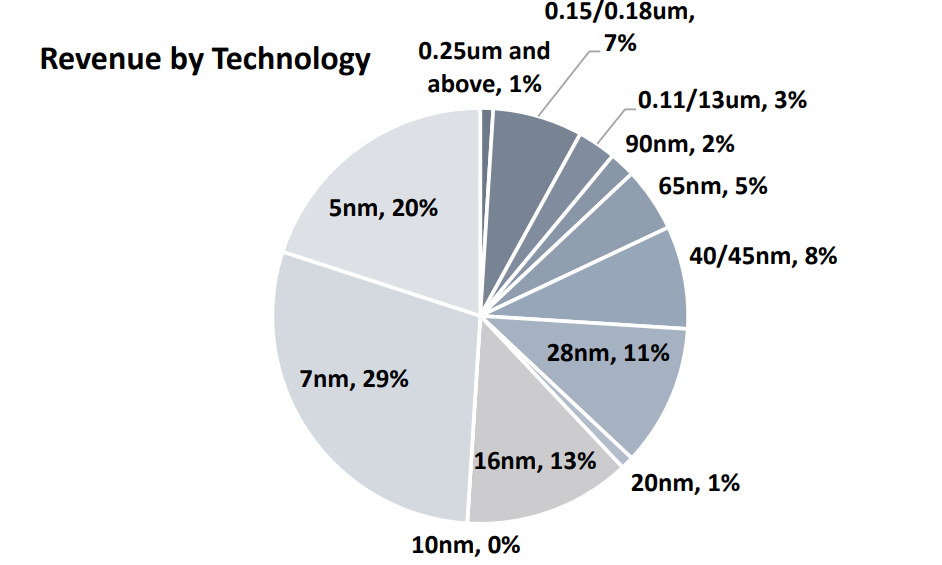
\includegraphics[width=0.9\linewidth]{RevenueByTechnology.png}
    \caption{TSMC revenue by technology. Source: \cite{TSMCInvestmentRecomendation}}
    \label{img:net-revenue-by-technology}
\end{wrapfigure}


Similarly to smartphone market, high performance computing market clients like AMD or NVIDIA require avant-garde production technologies.
Those clients usually produce bigger chips, that requires more mature production process, to achieve acceptable yields.
5 nm node is used to manufacture latest Apple products and HPC companies, despite of their size probably cannot outbid Apple for allocation.
For those reasons I think that HPC market probably constitutes most of 7 nm slice of figure \ref{img:net-revenue-by-technology}.

\begin{wrapfigure}{H}{0.7\textwidth}
    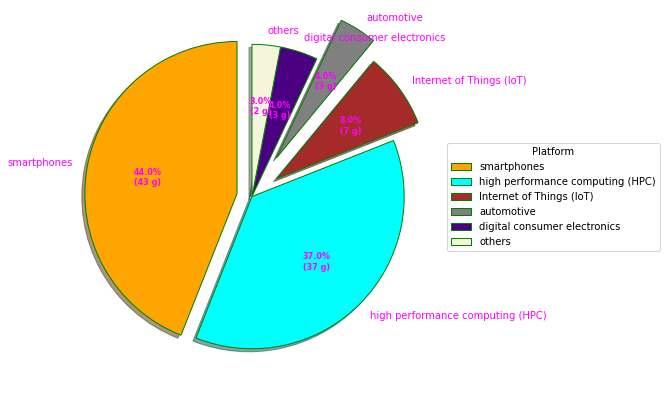
\includegraphics[width=0.9\linewidth]{net_revenue_by_platform.png}
    \caption{TSMC net revenue by platform. Data source: \cite{TSMCAnnualReport}}
    \label{img:net-revenue-by-platform}
\end{wrapfigure}


\subsection{Key Resources}
Mass production of semiconductors requires many highly specialised materials. 
Raw materials sourced from third party are shown in table \ref{tab:tsmc-suppliers}. 
As mentioned in introduction TSMC itself does not produce silicon wafers. 
TSMC wafers suppliers covers 90\% of world silicon wafer demand. 
Supplying wafers form multiple sources allows to keep mass production and alleviate supply risk.
Slurry, Pad, disk section of table \ref{tab:tsmc-suppliers} refers to CMP (Chemical Mechanical Polishing) technology. 
Some major suppliers of CMP and lithographic materials have relocated or plan to replicate their manufacturing sites closer to TSMC’s  facilities, thus significantly improving logistics and reducing supply risks. 

\begin{table}[H]
\begin{adjustbox}{max width=0.9\textwidth}
\begin{tabular}{@{}llll@{}}
\toprule
Materials                                & Suppliers                     & Materials                           & Suppliers                     \\ \midrule\midrule
                                         & FST                           & Gases                               & Air Liquide                   \\
                                         & GlobalWafers                  &                                     & Air Products                  \\
                                         & SEH                           &                                     & Central Glass                 \\
                                         & Siltronic                     &                                     & Entegris                      \\
                                         & SK siltron                    &                                     & Linde LienHwa                 \\
\multirow{-6}{*}{Raw Wafers}             & SUMCO                         &                                     & Praxair                       \\ \cmidrule(r){1-2}
                                         & Air Liquide                   &                                     & SK Materials                  \\
                                         & BASF                          &                                     & Taiwan Material Technology    \\
                                         & DuPont                        &                                     & Taiyo Nippon Sanso            \\ \cmidrule(l){3-4} 
                                         & Entegris                      &                                     & 3M                            \\
                                         & Fujifilm Electronic Materials &                                     & AGC                           \\
                                         & Kanto PPC                     &                                     & Cabot Microelectronics        \\
                                         & Kuang Ming                    &                                     & DuPont                        \\
                                         & Merck                         &                                     & Fujibo                        \\
                                         & RASA                          &                                     & Fujifilm Electronic Materials \\
                                         & Shiny                         & \multirow{-7}{*}{Slurry, Pad, Disk} & Fujim                         \\ \cmidrule(l){3-4} 
\multirow{-11}{*}{Chemicals}             & Tokuyama                      &                                     &                               \\ \cmidrule(r){1-2}
                                         & 3M                            &                                     &                               \\
                                         & Fujifilm Electronic Materials &                                     &                               \\
                                         & JSR                           &                                     &                               \\
                                         & Nissan                        &                                     &                               \\
                                         & Shin-Etsu Chemical            &                                     &                               \\
                                         & Sumitomo Chemical             &                                     &                               \\
\multirow{-7}{*}{Lithographic materials} & T.O.K.                        &                                     &                               \\ \cmidrule(r){1-2}
\end{tabular}
\end{adjustbox}
\caption{Materials used by TSMC by suppliers. Source \cite{TSMCAnnualReport}}
\label{tab:tsmc-suppliers}
\end{table}


% Water
% To make the most effective use of Taiwan’s limited water
% resources, all TSMC fabs strive to increase water reclamation
% rates by adjusting the water usage of manufacturing
% equipment and improving wastewater reclamation systems

%Litograpy machines

%Human resources



\subsection{Key Activities}
The main activities of TSMC company are manufacturing and engineering of the product, since whole R\&D process was made before order from the principal company.
TSMC has accumulated 50,000+ patents worldwide as of end of 2021, including 5,100 global patents received \cite{TSMCAnnualReport}.
As of the end of 2021, more than 1,900 Golden Trade Secret Awards have been granted and over 160,000 technical or commercial trade secrets have been registered on the trade secret registration.

\subsection{Key Partners}
% ASML - machines
TSMC operations and ongoing expansion plans depend on its ability to obtain an appropriate amount of equipment.
ASML is multinational lithography machine provider and the only company that provides extreme ultra violet (EUV) lithography equipment \cite{InsideASML}.
EUV lithography got its name from light source that is used print integrated circuits.
Single EUV machine costs around 200 million USD and is among the most complicated devices ever made.

Constant production requires constant flow of raw materials.
Breakdown of raw materials companies and their supplies can be found in table \ref{tab:tsmc-suppliers}. 
Every material is sourced from multiple companies, that can be consider a leader in their respective niche. 

\subsection{Cost Structure}

Comprehensive financial statements are included in annual report \cite{TSMCAnnualReport}, yet not a single direct cost source is mentioned. 
Therefore, compiling structure data from available sources vastly exceeds scope of this work. 


% Cost structure of TSMC is as follows:
% \begin{}
% \begin{itemize}
% \item three advanced 12-inch wafer GIGAFAB facilities
% \item four 8-inch wafer fabs
% \item one 6-inch wafer fab and two backend fabs
% \item cost of components and raw material
% \item quality control
% \item logistics and supply chain
% \item account management and engineering service offices
% \end{itemize}

\section{Conclusions}

This assignment profiles the biggest semiconductor suppliers in the world.
As public trade companies TSMC and many of its partners, reveal their internal processes and financial data as shareholder's information.
Those sources make writing this assignment possible.
TSMC operations can be described as any other production company. 
Company takes some raw materials, process them with some machines and sells them as new products to customers. 
What makes TSMC unique is scale of its operation and sci-fi level of tech that is used in its industrial units. 


\bibliographystyle{ieeetr}
\bibliography{refs} 

\end{document}
